 \documentclass[14pt, a4paper]{article} %14 pt indicates the font size of the prepared document
\usepackage[utf8]{inputenc} %indicates the encoding of the document
\usepackage{multicol}
\usepackage{multirow}
\usepackage{graphicx}
\usepackage{amsmath}
\usepackage{amsfonts} 
% or 
\usepackage{amssymb}
\usepackage{authblk}
\usepackage[document]{ragged2e}
\usepackage{geometry}

\title{CSE 300: Online Assignment}
\author{Md Shamsuzzoha Bayzid, Mahjabin Nahar, Md Shariful Islam Bhuyan and Md Saidur Rahman}
\date{June 2021}
\begin{document}
\maketitle

\section{Introduction}
This assignment has been designed to assess the preparation of the students in writing scientific articles using \LaTeX. This assignment covers a variety of components that are commonly used in scientific manuscripts.

    \subsection{Equations}
    Let $a_0$ $a_n$ and $b_n$ are the terms of a series. Therir definitions are given in Eqn. \ref{eq:1}.
    \newline
    \begin{flushleft}
     \begin{equation*}
        \begin{split}
        a_0 &= \frac{1}{\pi} \int^{-\pi}_{\pi} f(x) dx \\
        a_n &= \frac{1}{\pi} \int^{-\pi}_{\pi} cosnx dx = \frac{1}{\pi} \int^{-\pi}_{\pi} x^2 cosnx dx \\
        \end{split}
        \end{equation*}
        \begin{equation}\label{eq:1}
        \begin{split}
        b_n &= \frac{1}{\pi} \int^{-\pi}_{\pi} sinnx dx = \frac{1}{\pi} \int^{-\pi}_{\pi} x^2 sinnx dx \\
        \end{split}
        \end{equation}
    \end{flushleft}
    \subsection{Tables}
    We wish to place the Table at the bottom of the page.
    \subsection{Figures}
    We intend to put Figure \ref{fig:1} at the top of a page.\pagebreak
    \begin{figure}[t!]
        \centering
        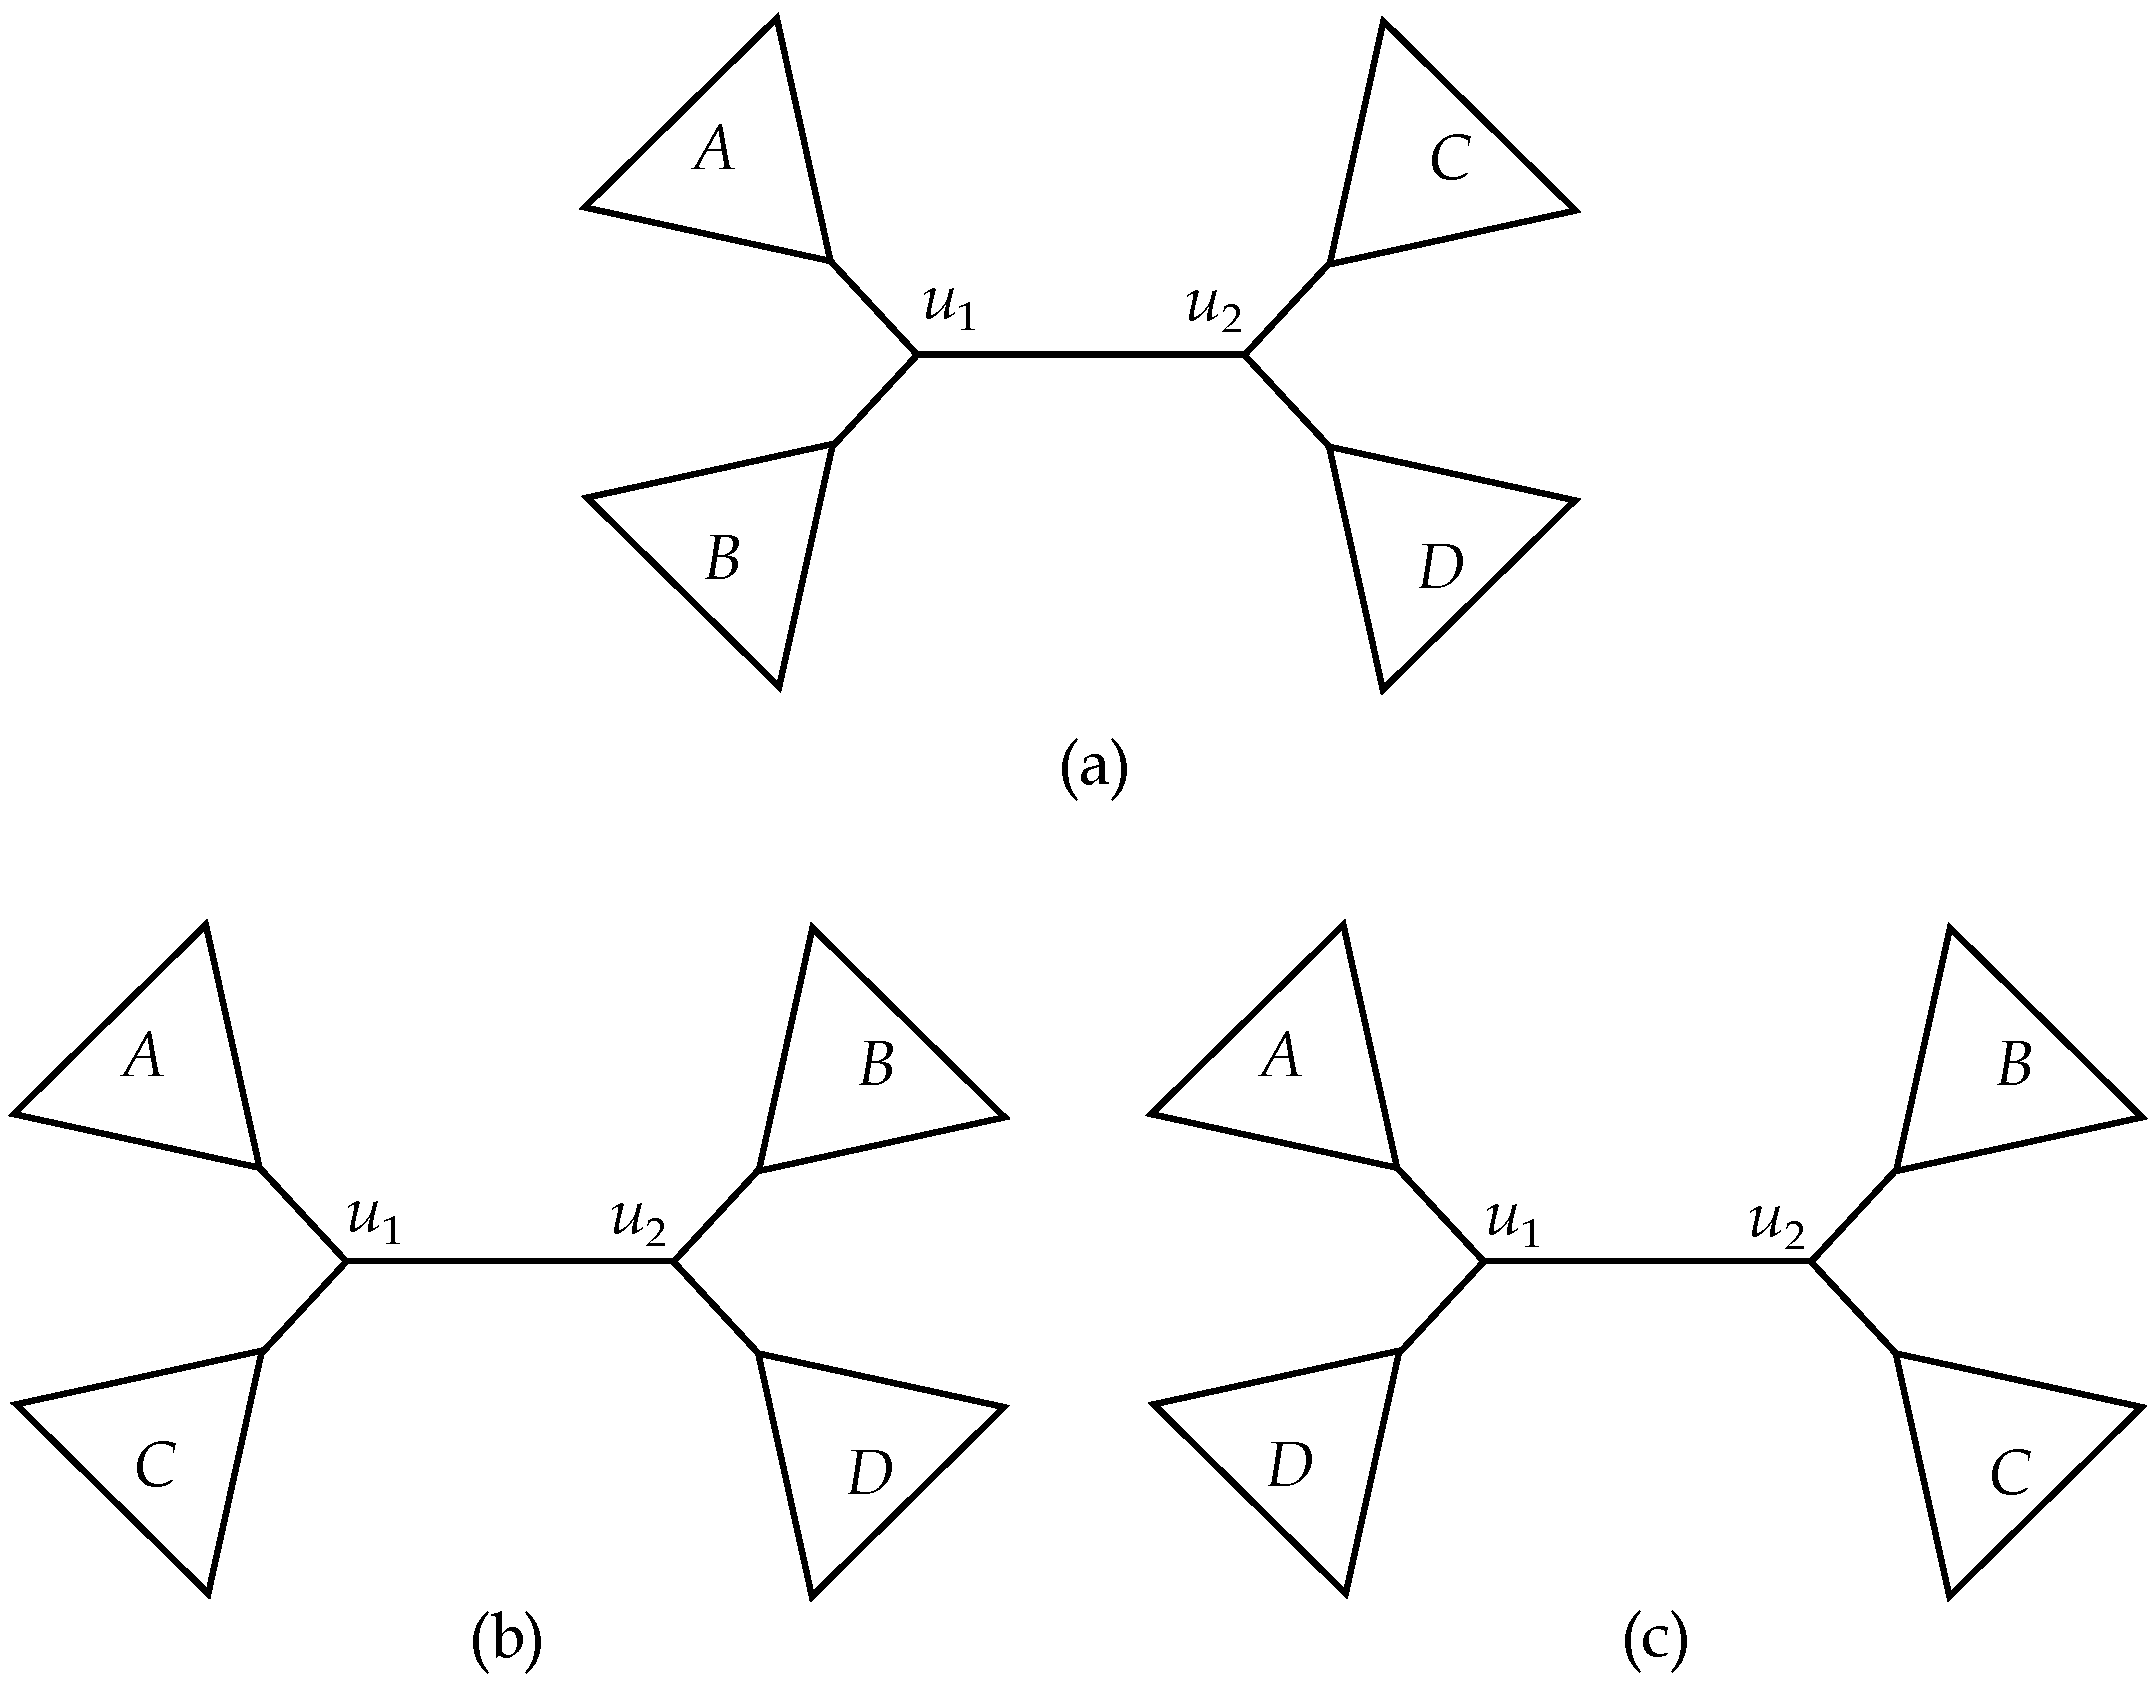
\includegraphics[width=0.75\linewidth]{Figure3.pdf}
        \caption{\label{fig:1}\textbf{Side by side same figure}}
    \end{figure}
\section{Conclusions}
The major objectives of this assignment are listed below (please do not ignore the font sizes)
    \begin{itemize}
     \item {\huge{To assess the ability of the students in preparing manuscripts in \LaTeX}}
     \item {\large{To see if the students have adequately practiced different aspects of writing in \LaTeX}}
\begin{table}[b]
\begin{tabular}{|llc||ccc|cll|l|l|lll|}
\hline
\multicolumn{14}{|c|}{Item List}                                                                                                                                                                                \\ \hline
Item    & Name                 & or & \multicolumn{3}{c|}{\multirow{2}{*}{ALPHA 2 Code}} & \multicolumn{3}{l|}{\multirow{2}{*}{ALPHA 3 Code}} & \multicolumn{5}{l|}{\multirow{2}{*}{Numerical Code}}            \\
\multicolumn{3}{|l||}{Product Name}  & \multicolumn{3}{c|}{}                              & \multicolumn{3}{l|}{}                              & \multicolumn{5}{l|}{}                                           \\ \hline
Item001 & \multicolumn{1}{c}{} &    & AF               &                &                & AFG               &                &               &  & 004 &                          &                          &  \\ \cline{11-11}
Item002 &                      &    & AX               &                &                & ALA               &                &               &  & 008 &                          &                          &  \\ \cline{11-11}
Item003 & \multicolumn{1}{c}{} &    & AL               &                &                & ALB               &                &               &  & 009 &                          &                          &  \\ \cline{11-13}
Item004 &                      &    & DZ               &                &                & DZA               &                &               &  & 012 & \multicolumn{1}{l|}{013} & \multicolumn{1}{l|}{014} &  \\ \hline \hline
Item005 & \multicolumn{1}{c}{} &    & AS               &                &                & ASM               &                &               &  & 016 &                          &                          &  \\ \cline{11-12}
Item006 &                      &    & AD               &                &                & AND               &                &               &  & 010 & \multicolumn{1}{l|}{020} &                          &  \\ \cline{11-12}
Item007 &                      &    & AO               &                &                & AGO               &                &               &  & 024 & \multicolumn{1}{l|}{025} &                          &  \\ \hline \hline \hline
\end{tabular}
\end{table}
\pagebreak
    \item{To see if the students can add various basic components (e.g., tables, figures, equations) to a \LaTeX manuscript.
}
    \item{\small{To see if the students can leverage the available materials (both offline and online) to do something which has not explicitly been taught in the class.}}
    \end{itemize}
\end{document}
